\documentclass{article}
\usepackage{amsmath}
\usepackage{amssymb}
\usepackage{graphicx}
\usepackage{enumitem}
\usepackage[utf8]{inputenc}
\graphicspath{{Imagenes/}}

\title{\Huge Taller de Herramientas Computacionales}
\author {Diego Armando Santillán Arriaga}
\date{15/enero/19}
	
\begin{document}
\maketitle
	\begin{center}
		%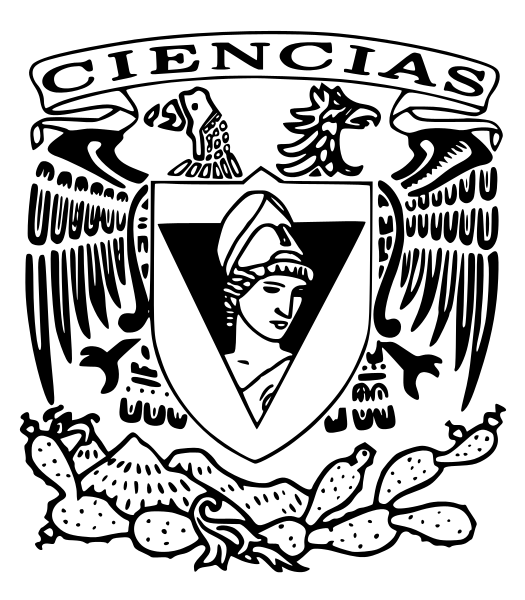
\includegraphics[scale=0.40]{1.png}
	\end{center}
\newpage

%\section{Expresiones matemáticas}: sin asterisco aparece el número de sección.
\section*{Expresiones matemáticas}
$\alpha + \beta$\\ %\(\)
\[\alpha + \beta\] %Con corchetes se centra el texto en la línea siguiente

\subsection{Índices y subíndices}
$x_{2}$
$x^2$\\

\section{fracciones y divisiones etc}
$\frac{2}{2}$
$\frac{\frac{3}{4}}{\frac{2}{3}}$

\section{raiz cuadrada y potencias}
$\sqrt{2} + \sqrt{3^2}^2$

$\int {a}^{b} x^2 \partial$
%x^2$\\\begin{equation}\label{key}

%\end{equation}

$3 \quad 2$


\section*{Matrices}
%\dots puntos suspensivos
%\vdots puntos suspensivos verticales
\[
\begin{bmatrix}
x_{2} & x_{3}\\
x_{4} & x_{6}
\end{bmatrix}
\]
\[
\begin{bmatrix}
x_{2} & x_{5} & \dots\\
x_{5} & x_{20} &\vdots\\
\vdots & \vdots & \vdots
 
\end{bmatrix}\]
$\sum$

\section*{Tablas}

\[
\begin{array}{|c|c|c|}
\hline
f(t) & F(s) & \mbox{Remark}\\
\hline\hline
\delta(t) & 1 & \mbox{unit step function}\\
u(t) & \frac{1}{s} & \mbox{unit step function}\\
e^{at}u(t) & \frac{1}{s-a} & \mbox{one side exponential}\\
\hline\end{array}\]

\section*{Alineamiento}


\end{document}





